Dadas a complexidade e heterogeneidade de ambientes de computação em nuvem, que possuem inúmeros componentes e variáveis dinâmicas interligadas que necessitam ser orquestradas, a gerência destes ambientes torna-se humanamente impossível \cite{forecasting}. Tendo isso em vista, ferramentas foram criadas com o objetivo de orquestrar a infraestrutura do ambiente, realizando a ligação dos diferentes componentes como servidores de armazenamento, virtualização e dispositivos de redes para prover a abstração de uma nuvem computacional.

\citeonline{tcc-gabriel} cita cinco componentes que compõe as ferramentas disponíveis para orquestração:
\begin{enumerate} 
 \item Um gerente de identidades que realiza a gerência das credenciais dos usuários (autenticação e autorização), possibilitando maior segurança na organização da infraestrutura;
 \item Um gerente de alocação que aloca máquinas virtuais quando são instanciadas, ligadas ou migradas;
 \item Um \emph{hypervisor} que é o componente que interage com diferentes virtualizadores, sendo responsável por enviar comandos e gerenciar cada cluster;
 \item Um componente de armazenamento que realiza a distribuição e o compartilhamento dos HDs de máquinas virtuais entre os servidores;
 \item Um elemento encarregado de gerenciar a configuração da rede.
\end{enumerate}

A Figura \ref{fig:orquestracao}, retirada desse estudo, mostra de forma visual a arquitetura de uma ferramenta de orquestração.

 \begin{figure}[!htb]
 	\centering
 	\caption{Representação de uma ferramenta de orquestração \cite{tcc-gabriel}.}\label{fig:orquestracao}
 	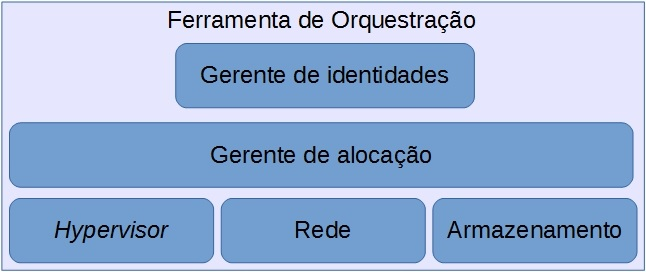
\includegraphics[width=1\textwidth]{figuras/ferramentasOrquestracao.jpg}
 \end{figure}
 
A ferramenta escolhida por \citeonline{tcc-gabriel} e a qual será utilizada no desenvolvimento deste trabalho é o CloudStack \cite{cloudstack}. A escolha se dá aos motivos de que a ferramenta demonstra uma evolução constante num projeto que mantém uma comunidade participativa, documentação completa e detalhada e o uso de tecnologias conhecidas para armazenamento de dados.
